\documentclass[survey]{cpecmu}

%% This is a sample document demonstrating how to use the CPECMU
%% project template. If you are having trouble, see "cpecmu.pdf" for
%% documentation.

\projectNo{P069-1}
\acadyear{2025}

\titleTH{สื่อการสอนคณิตศาสตร์ประเภท sandbox สำหรับนักเรียนชั้นประถมปลาย}
\titleEN{Mathematical learning sandbox for upper primary school students}

\author{นายธนภัทร เชยชมศรี}{TANAPAT CHOEICHOMSRI}{650610767}
\author{นายธีรภัทร์ ลำตาล}{THEERAPAT LUMTAN}{650610772}
\author{นางสาวพนิดา สุทธภักติ}{PANIDA SUTHAPAKTI}{650610790}
\author{นายอนรรฆ สันตินรนนท์}{ANAK SARNTINORANONT}{650610817}

\cpeadvisor{chinawat}
\cpecommittee{thanatip}
\committee{รศ.ดร.\,นิพนธ์ ธีรอำพน}{Assoc.\,Prof.\,Nipon Theera-Umpon, Ph.D.}
\committee{ดร.\,พรรณชมพู วิสิฐธนวรรธ}{Dr.\,Pannachompoo Wisitthananon}
\committee{ผศ.ดร.\,ศุภณัฐ ชัยดี}{Asst.\,Prof.\,Supanat Chaidee, Ph.D.}

%% Some possible packages to include:
\usepackage[final]{graphicx} % for including graphics

%% Add bookmarks and hyperlinks in the document.
\PassOptionsToPackage{hyphens}{url}
\usepackage[colorlinks=true,allcolors=Blue4,citecolor=red,linktoc=all]{hyperref}
\def\UrlLeft#1\UrlRight{$#1$}

%% Needed just by this example, but maybe not by most reports
\usepackage{afterpage} % for outputting
\usepackage{pdflscape} % for landscape figures and tables. 

%% Some other useful packages. Look these up to find out how to use
%% them.
% \usepackage{natbib}    % for author-year citation styles
% \usepackage{txfonts}
% \usepackage{appendix}  % for appendices on a per-chapter basis
% \usepackage{xtab}      % for tables that go over multiple pages
% \usepackage{subfigure} % for subfigures within a figure
% \usepackage{pstricks,pdftricks} % for access to special PostScript and PDF commands
% \usepackage{nomencl}   % if you have a list of abbreviations

%% if you're having problems with overfull boxes, you may need to increase
%% the tolerance to 9999
% \tolerance=9999

\bibliographystyle{plain}
% \bibliographystyle{IEEEbib}

% \renewcommand{\topfraction}{0.85}
% \renewcommand{\textfraction}{0.1}
% \renewcommand{\floatpagefraction}{0.75}

%% Example for glossary entry
%% Need to use glossary option
%% See glossaries package for complete documentation.
\ifglossary
  \newglossaryentry{lorem ipsum}{
    name=lorem ipsum,
    description={derived from Latin dolorem ipsum, translated as ``pain itself''}
  }
\fi

%% Uncomment this command to preview only specified LaTeX file(s)
%% imported with \include command below.
%% Any other file imported via \include but not specified here will not
%% be previewed.
%% Useful if your report is large, as you might not want to build
%% the entire file when editing a certain part of your report.
% \includeonly{chapters/intro,chapters/background}

\begin{document}
\maketitle
\makesignature

\ifproject
\begin{abstractTH}
ในปัจจุบัน การเรียนรู้เรื่อง “เศษส่วน” สำหรับนักเรียนระดับประถมศึกษายังคงเป็นเรื่องที่เข้าใจได้ยาก เนื่องจากเป็นแนวคิดเชิงนามธรรมที่นักเรียนไม่คุ้นเคย และสื่อการสอนที่มีอยู่ส่วนใหญ่มักมุ่งเน้นการผลลัพธ์ เช่น การหาคำตอบที่ถูกต้องหรือการทำโจทย์ให้ได้คะแนน มากกว่าการสร้างความเข้าใจในหลักการและกระบวนการคิด ทำให้นักเรียนไม่สามารถเชื่อมโยงเศษส่วนกับสถานการณ์ในชีวิตจริงได้

ด้วยเหตุนี้ ผู้จัดทำจึงเสนอแนวคิดในการพัฒนาสื่อการสอนแบบเปิด เพื่อให้นักเรียนได้ลงมือทดลอง คิดแก้ปัญหา และค้นพบความรู้ด้วยตนเองผ่านการจำลองสถานการณ์ต่าง ๆ ที่เกี่ยวข้องกับเศษส่วน โดยเน้นให้เด็กได้สังเกตและเข้าใจแนวคิดหลักโดยไม่ถูกจำกัดด้วยวิธีการคงที่หรือตัวเลือกที่ตายตัว ซึ่งจะเป็นประโยชน์ต่อทั้งนักเรียน และครูที่จะได้เครื่องมือช่วยสอนที่มีประสิทธิภาพ สอดคล้องกับหลักสูตร

โดยแนวทางที่เลือกใช้คือการออกแบบและพัฒนาสื่อการสอนเชิงโต้ตอบที่เน้นการสะท้อนสถานการณ์จริง เช่น การวัดพื้นที่ การแบ่งสิ่งของ ในส่วนของทางเลือกอื่นที่พิจารณาแทนได้คือ การใช้สื่อเทคโนโลยี เช่น แอปพลิเคชันหรือเกม รวมทั้งการใช้สื่อวิดีโอและภาพเคลื่อนไหว

เงื่อนไขและข้อจำกัดที่มีได้แก่ ความครอบคลุมของเนื้อหาที่ต้องจำเพาะเจาะจงไปที่เนื้อหาเรื่องเศษส่วนเพียงเรื่องเดียว เพราะเป็นเรื่องที่เด็กต้องใช้เวลาในการเชื่อมโยงเพื่อเข้าใจหลักการของเศษส่วนอย่างแท้จริง นอกจากนี้ สื่อการสอนนี้อาจเป็นสื่อที่แปลกใหม่สำหรับครูผู้สอน จึงจำเป็นต้องมีการแนะแนวหรือจัดทำคู่มือเพื่อให้การใช้งานมีประสิทธิภาพ
\end{abstractTH}

\begin{abstract}
At present, learning about fractions for elementary school students remains difficult to understand, as it is an abstract concept that students are not familiar with. Most of the existing teaching materials tend to focus on outcomes—such as finding the correct answers or solving problems to earn scores—rather than fostering understanding of the principles and thought processes. This results in students being unable to connect fractions with real-life situations.

For this reason, the author proposes the idea of developing open-ended teaching materials, allowing students to experiment, think critically, solve problems, and discover knowledge by themselves through simulations of various situations related to fractions. The focus is on encouraging children to observe and grasp the core concepts without being constrained by fixed methods or predetermined choices. This approach would benefit both students—by supporting deeper understanding—and teachers—by providing an effective teaching tool aligned with the curriculum.

The chosen approach is to design and develop interactive teaching materials that reflect real-world situations, such as measuring areas or dividing objects. Alternative options considered include using technology-based media such as applications or games, as well as video and animation media.

The conditions and limitations include the scope of the content, which must specifically focus only on fractions, since students need time to build connections and gain a true understanding of fraction principles. Moreover, because this teaching material may be new to teachers, it is necessary to provide guidance or manuals to ensure effective use.
\end{abstract}

\iffalse
\begin{dedication}
This document is dedicated to all Chiang Mai University students.

Dedication page is optional.
\end{dedication}
\fi % \iffalse

\begin{acknowledgments}
Your acknowledgments go here. Make sure it sits inside the
\texttt{acknowledgment} environment.

\acksign{2020}{5}{25}
\end{acknowledgments}%
\fi % \ifproject

\contentspage

\ifproject
\figurelistpage

\tablelistpage
\fi % \ifproject

% \abbrlist % this page is optional

% \symlist % this page is optional

% \preface % this section is optional


\pagestyle{empty}\cleardoublepage
\normalspacing \setcounter{page}{1} \pagenumbering{arabic} \pagestyle{cpecmu}

\chapter{\ifenglish Introduction\else บทนำ\fi}
ในปัจจุบัน การเรียนรู้เรื่อง “เศษส่วน” สำหรับนักเรียนระดับประถมศึกษายังคงเป็นเรื่องที่เข้าใจได้ยาก เนื่องจากเป็นแนวคิดเชิงนามธรรมที่นักเรียนไม่คุ้นเคย และสื่อการสอนที่มีอยู่ส่วนใหญ่มักมุ่งเน้นการผลลัพธ์ เช่น การหาคำตอบที่ถูกต้องหรือการทำโจทย์ให้ได้คะแนน มากกว่าการสร้างความเข้าใจในหลักการและกระบวนการคิด ทำให้นักเรียนไม่สามารถเชื่อมโยงเศษส่วนกับสถานการณ์ในชีวิตจริงได้

ด้วยเหตุนี้ ผู้จัดทำจึงเสนอแนวคิดในการพัฒนาสื่อการสอนแบบเปิด เพื่อให้นักเรียนได้ลงมือทดลอง คิดแก้ปัญหา และค้นพบความรู้ด้วยตนเองผ่านการจำลองสถานการณ์ต่างๆ ที่เกี่ยวข้องกับเศษส่วน โดยเน้นให้เด็กได้สังเกตและเข้าใจแนวคิดหลักโดยไม่ถูกจำกัดด้วยวิธีการคงที่หรือตัวเลือกที่ตายตัว

\section{\ifenglish Project rationale\else ที่มาของโครงงาน\fi}
\begin{enumerate}
    \item นักเรียนระดับประถมศึกษายังมีความเข้าใจในเรื่องเศษส่วนไม่มากนัก โดยนักเรียนสามารถบอกได้เพียงว่าเศษส่วนคืออะไร แต่ไม่สามารถอธิบายความหมายออกมาได้
    \item สื่อการสอนที่มีอยู่ยังไม่ตอบโจทย์การเรียนรู้ของนักเรียน
\end{enumerate}

\section{\ifenglish Objectives\else วัตถุประสงค์ของโครงงาน\fi}
\begin{enumerate}
    \item สร้าง Web Application เชิงโต้ตอบ (Interactive) สำหรับการเรียนรู้ในเรื่องของเศษส่วน เกี่ยวกับความเข้าใจเบื้องต้น การบวก และการลบ โดยใช้ Length model
    \item สร้างเครื่องมือการเรียนรู้ ที่ให้ผู้เรียนสามารถทดลอง แบ่ง แทนค่า และจัดการเศษส่วนด้วยภาพ
\end{enumerate}

\section{\ifenglish Project scope\else ขอบเขตของโครงงาน\fi}
โครงงานจะสร้างเป็น Web Application เชิงโต้ตอบ (Interactive) สำหรับการเรียนรู้ในเรื่องของเศษส่วน เกี่ยวกับความเข้าใจเบื้องต้น การบวก และการลบ โดยใช้ Length model

\subsection{\ifenglish Hardware scope\else ขอบเขตด้านฮาร์ดแวร์\fi}
โครงงานนี้จะมุ่งเน้นการพัฒนาซอฟต์แวร์ที่สามารถใช้งานบนโทรศัพท์มือถือเป็นหลัก

\subsection{\ifenglish Software scope\else ขอบเขตด้านซอฟต์แวร์\fi}
โครงงานนี้จะพัฒนาเป็น Web Application ที่ไม่จำเป็นต้องติดตั้งโปรแกรมเพิ่มเติมใดๆ โดยสามารถใช้งานผ่านเว็บเบราว์เซอร์ได้ทันที กล่าวคือเพียงแค่มีสัญญาณอินเทอร์เน็ตก็สามารถใช้งานได้

\section{\ifenglish Expected outcomes\else ประโยชน์ที่ได้รับ\fi}
\begin{enumerate}
    \item นักเรียนชั้นประถมปลายมีความเข้าใจเรื่องเศษส่วนมากขึ้น
    \item มีช่องทางในการศึกษาเศษส่วนเพิ่มขึ้น
\end{enumerate}

\section{\ifenglish Technology and tools\else เทคโนโลยีและเครื่องมือที่ใช้\fi}

\subsection{\ifenglish Hardware technology\else เทคโนโลยีด้านฮาร์ดแวร์\fi}

\subsection{\ifenglish Software technology\else เทคโนโลยีด้านซอฟต์แวร์\fi}

\section{\ifenglish Project plan\else แผนการดำเนินงาน\fi}

\begin{plan}{6}{2025}{12}{2025}
    \planitem{6}{2025}{8}{2025}{Project research}
    \planitem{9}{2025}{9}{2025}{Requirements elicitation}
    \planitem{10}{2025}{10}{2025}{Design}
\end{plan}

\section{\ifenglish Roles and responsibilities\else บทบาทและความรับผิดชอบ\fi}
อธิบายว่าในการทำงาน นศ. มีการกำหนดบทบาทและแบ่งหน้าที่งานอย่างไรในการทำงาน จำเป็นต้องใช้ความรู้ใดในการทำงานบ้าง

\section{\ifenglish%
Impacts of this project on society, health, safety, legal, and cultural issues
\else%
ผลกระทบด้านสังคม สุขภาพ ความปลอดภัย กฎหมาย และวัฒนธรรม
\fi}
งานวิจัยนี้มีผลกระทบในด้านต่างๆ ดังนี้
\begin{enumerate}
    \item ด้านสังคม: นักเรียนชั้นประถมปลายมีความเข้าใจเรื่องเศษส่วนมากขึ้น ส่งผลให้มีความสนใจและมีทัศนคติที่ดีในวิชาคณิตศาสตร์
    \item ด้านสุขภาพ: ช่วยลดความเครียดจากการเรียนการสอนคณิตศาสตร์ ทั้งในตัวนักเรียนและครูผู้สอน
\end{enumerate}

แนวทางและโยชน์ในการประยุกต์ใช้งานโครงงานกับงานในด้านอื่นๆ รวมถึงผลกระทบในด้านสังคมและสิ่งแวดล้อมจากการใช้ความรู้ทางวิศวกรรมที่ได้

\chapter{\ifenglish Background Knowledge and Theory\else ทฤษฎีที่เกี่ยวข้อง\fi}

การทำโครงงาน เริ่มต้นด้วยการศึกษาค้นคว้า ทฤษฎีที่เกี่ยวข้อง หรือ งานวิจัย/โครงงาน ที่เคยมีผู้นำเสนอไว้แล้ว ซึ่งเนื้อหาในบทนี้ก็จะเกี่ยวกับการอธิบายถึงสิ่งที่เกี่ยวข้องกับโครงงาน เพื่อให้ผู้อ่านเข้าใจเนื้อหาในบทถัดๆ ไปได้ง่ายขึ้น

\section{Fraction models}
ลักษณะของเศษส่วนที่ใช้สื่อความหมายมีหลายแบบ เช่น โดยแต่ละแบบมีจุดเด่นที่แตกต่างกันไป

\subsection{Area model}
Area model เป็นการใช้รูปทรงเรขาคณิตต่างๆ เช่น วงกลม สี่เหลี่ยม หรือรูปสามเหลี่ยม มาแบ่งส่วนเพื่อแสดงความหมายของเศษส่วน
\begin{figure}[h!tbp]
\begin{centering}
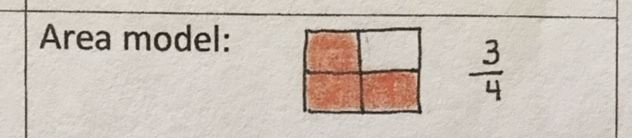
\includegraphics{Area_model.png}
\end{centering}
\caption[Area model]{Area model of fraction 3/4}
\end{figure}

\subsection{Set model}
Set model เป็นการใช้กลุ่มของวัตถุที่เหมือนกันมาแบ่งกลุ่มเพื่อแสดงความหมายของเศษส่วน เช่น การใช้ลูกปัดสีแดงและสีขาวมาแบ่งกลุ่มเพื่อแสดงเศษส่วน
\begin{figure}[h!tbp]
\begin{center}
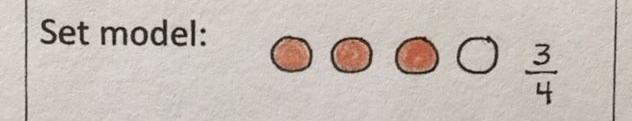
\includegraphics{Set_model.png}
\end{center}
\caption[Set model]{Set model of fraction 3/4}
\end{figure}

\subsection{Length model}
Length model เป็นการใช้เส้นตรงเพื่อแสดงความหมายของเศษส่วน โดยจะเป็นการใช้เส้นตรงยาว 1 หน่วยมาแบ่งเป็นส่วนๆ
\begin{figure}[h!tbp]
\begin{center}
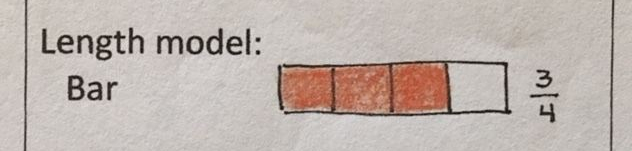
\includegraphics{Length_model.png}
\end{center}
\caption[Length model]{Length model of fraction 3/4}
\end{figure}


% This code demonstrates how to get a landscape table or figure. It
% uses the package lscape to turn everything but the page number into
% landscape orientation. Everything should be included within an
% \afterpage{ .... } to avoid causing a page break too early.


\section{\ifenglish%
\ifcpe CPE \else ISNE \fi knowledge used, applied, or integrated in this project
\else%
ความรู้ตามหลักสูตรซึ่งถูกนำมาใช้หรือบูรณาการในโครงงาน
\fi
}

ความรู้จากหลักสูตรวิชา Software Engineering โดยมีการใช้ความรู้ในเรื่องของการวิเคราะห์และออกแบบระบบซอฟต์แวร์ รวมไปถึงการพัฒนาระบบและการแบ่งงานในทีม ซึ่งความรู้เหล่านี้ถูกนำมาใช้หรือบูรณาการในโครงงาน

\section{\ifenglish%
Extracurricular knowledge used, applied, or integrated in this project
\else%
ความรู้นอกหลักสูตรซึ่งถูกนำมาใช้หรือบูรณาการในโครงงาน
\fi
}

\begin{itemize}
    \item place here
\end{itemize}

\chapter{\ifproject%
\ifenglish Project Structure and Methodology\else โครงสร้างและขั้นตอนการทำงาน\fi
\else%
\ifenglish Project Structure\else โครงสร้างของโครงงาน\fi
\fi
}

ในบทนี้จะกล่าวถึงขั้นตอนการดำเนินงานในโครงงานนี้

\makeatletter

% \renewcommand\section{\@startsection {section}{1}{\z@}%
%                                    {13.5ex \@plus -1ex \@minus -.2ex}%
%                                    {2.3ex \@plus.2ex}%
%                                    {\normalfont\large\bfseries}}

\makeatother
%\vspace{2ex}
% \titleformat{\section}{\normalfont\bfseries}{\thesection}{1em}{}
% \titlespacing*{\section}{0pt}{10ex}{0pt}

\section{การค้นคว้าข้อมูล}
ในช่วงเริ่มต้นของโครงงานนี้ จะเป็นการค้นคว้าข้อมูลที่เกี่ยวข้องกับโครงงานนี้ เพื่อให้เข้าใจถึงปัญหาและ\\
แนวทางการแก้ไขปัญหาที่มีอยู่ในปัจจุบัน

\subsection{วิเคราะห์ปัญหา}
 เริ่มจากการตั้งข้อสงสัยว่า การเรียนรู้วิชาคณิตศาสตร์เรื่องเศษส่วนสำหรับเด็กนักเรียนชั้นประถมศึกษาในปัจจุบันนั้นมีปัญหาอย่างไรบ้าง
 หลังจากนั้นเราได้ติดต่อพูดคุยกับเจ้าหน้าที่ของ สสวท. เพื่อสอบถามเกี่ยวกับข้อสงสัยนี้และได้ข้อมูลว่า การเรียนรู้วิชาคณิตศาสตร์เรื่องเศษส่วนนั้นเป็นปัญหาที่พบในเด็กนักเรียนชั้นประถมศึกษาทั่วโลก
 เนื่องจากเนื้อหาในเรื่องนี้มีความเป็นนามธรรมที่สูง มีรูปแบบจำนวนที่ต่างจากคณิตศาสตร์ในเรื่องก่อนๆ และอาจมีหลักการที่ดูขัดแย้งกับสิ่งที่เขาเคยเรียนมา จึงยากที่จะทำให้เด็กทุกคนเข้าใจพร้อมๆกันและไม่สามารถทำเด็กทุกคนเข้าใจเรื่องนี้ด้วยวิธีสอนเดียวกันได้

\subsection{วิเคราะห์วิธีแก้ปัญหาที่มีอยู่ในปัจจุบัน}
จากการวิเคราะห์ปัญหาที่พบ จะพบได้ว่า วิธีการแก้ปัญหาที่มีอยู่ในปัจจุบันนั้น ยังไม่สามารถแก้ไขปัญหาได้อย่างตรงจุด
 เนื่องจากวิธีการสอนในปัจจุบันยังคงเป็นการสอนแบบท่องจำและมีสื่อประกอบในรูปแบบของ Area Model เพียงอย่างเดียว
 ทำให้เด็กนักเรียนไม่เข้าใจในความหมายของเศษส่วน และวิธีการนำไปใช้ในชีวิตประจำวัน
 
\subsection{สรุปปัญหาเบื้องต้น}
ปัญหาที่พบจากการวิเคราะห์ปัญหาและวิธีแก้ปัญหาที่มีอยู่ในปัจจุบัน คือ เด็กนักเรียนยังไม่เข้าใจในความหมายของเศษส่วน
 และไม่สามารถนำความรู้ที่ได้ไปใช้ในชีวิตประจำวันได้ แม้จะมีสื่อประกอบการสอนในรูปแบบของ Area Model ก็ตาม

\section{การลงพื้นที่สำรวจ}

\subsection{เลือกพี้นที่สำรวจ}
กลุ่มของเราได้เลือกโรงเรียนที่มีการสอนนักเรียนระดับชั้นประถมศึกษาตอนปลายในเขตเชียงใหม่ทั้งสิ้น 6 โรงเรียน ได้แก่ โรงเรียนพิงครัตน์, โรงเรียนพุทธิโศภน, โรงเรียนดาราวิทยาลัย, โรงเรียนบ้านเชิงดอยสุเทพ, โรงเรียนโกวิทธำรงเชียงใหม่ และโรงเรียนสาธิตมหาวิทยาลัยเชียงใหม่
 ซึ่งแต่ละโรงเรียนนั้นมีระยะทางที่ไม่ไกลจากมหาวิทยาลัยเชียงใหม่มากนักและสามารถทำการติดต่อขออนุญาตจากทางโรงเรียนได้

\subsection{วางแผนออกสำรวจ}
การออกไปสำรวจในแต่ละโรงเรียนนั้น เราได้ทำการสัมภาษณ์ครูผู้สอนวิชาคณิตศาสตร์จำนวน 1-2 คน และนักเรียนจำนวน 6 คน
 เพื่อทำการสำรวจปัญหาที่เกิดขึ้นในการเรียนการสอนวิชาคณิตศาสตร์เรื่องเศษส่วน
% \include{chapters/eval}
\ifproject
\chapter{\ifenglish Conclusions and Discussions\else บทสรุปและข้อเสนอแนะ\fi}

\section{\ifenglish Conclusions\else สรุปผล\fi}

ข้อจำกัดในการทำโปรเจกต์นี้ คือจำเป็นต้องทำการคำนึงถึงเนื้อหาที่เหมาะสมกับกลุ่มเป้าหมายเป็นหลักอยู่เสมอ รวมถึงการออกแบบ UX/UI ที่ผู้ใช้สามารถใช้งานได้จริง นอกจากนี้ยังมีปัจจัยด้านเวลาที่จำกัด ส่งผลให้ฟังก์ชั่นที่เลือกทำนั้นมีได้จำกัด

\section{\ifenglish Challenges\else ปัญหาที่พบและแนวทางการแก้ไข\fi}

ในการทำโครงงานนี้ พบว่าเกิดปัญหาหลักๆ ดังนี้
\begin{itemize}
    \item การออกแบบ UX/UI: ที่เหมาะสมกับกลุ่มเป้าหมาย เนื่องจากกลุ่มเป้าหมายเป็นนักเรียนระดับประถม การออกแบบต้องคำนึงถึงความง่ายในการใช้งานและความน่าสนใจ เพื่อให้เด็กๆรู้สึกอยากใช้งานแอปพลิเคชัน
    \item การเลือกเนื้อหาที่เหมาะสม: เนื้อหาที่นำเสนอในแอปพลิเคชันต้องสอดคล้องกับหลักสูตรการเรียนรู้ของเด็กนักเรียน และต้องมีความน่าสนใจเพื่อกระตุ้นความสนใจในการเรียนรู้
    \item การจัดการเวลา: เนื่องจากเวลาที่มีจำกัด จึงต้องมีการวางแผนการทำงานอย่างมีประสิทธิภาพ เพื่อให้สามารถพัฒนาแอปพลิเคชันได้ตามเป้าหมายที่ตั้งไว้
\end{itemize}

\section{\ifenglish%
Suggestions and further improvements
\else%
ข้อเสนอแนะและแนวทางการพัฒนาต่อ
\fi
}

ข้อเสนอแนะเพื่อพัฒนาโครงงานนี้ต่อไป มีดังนี้
\begin{itemize}
    \item เพิ่มขอบเขตเนื้อหา โดยขยายขอบเขตเนื้อหาที่ครอบคลุมมากขึ้น เช่น การคูณและการหารเศษส่วน เพื่อให้ผู้เรียนได้รับความรู้ที่หลากหลายมากขึ้น
    \item เพิ่มฟีเจอร์การติดตามความก้าวหน้า โดยพัฒนาระบบที่ช่วยให้ผู้เรียนสามารถติดตามความก้าวหน้าในการเรียนรู้ของตนเองได้ เช่น การบันทึกคะแนนหรือการแสดงผลการทำแบบฝึกหัด 
\end{itemize}
\fi

\bibliography{report}

\ifproject
\normalspacing
\appendix
\chapter{กระบวนการสอนเนื้อหาเรื่องเศษส่วนให้กับเด็ก}

\sloppy เอกสารนี้เป็นส่วนเสริมในภาคผนวก ซึ่งจะกล่าวถึงการสอนเนื้อหาเรื่องเศษส่วนให้กับเด็กในต่างประเทศ

\section{การสอนเนื้อหาเรื่องเศษส่วน}

การสอนเนื้อหาเรื่องเศษส่วนให้กับเด็กนั้น มีหลายวิธีการที่สามารถนำมาใช้ได้ เช่น การใช้ภาพประกอบ การใช้วัตถุจริง โดยสำหรับเด็กที่พึ่งเริ่มเรียนรู้เรื่องเศษส่วนนั้น การใช้ Fraction Model ที่เป็น Length Model จะช่วยให้เด็กเข้าใจแนวคิดของเศษส่วนได้ง่ายมากกว่า Model อื่นๆ

\section{ความยากของเนื้อหาเรื่องเศษส่วน}

เนื้อหาเรื่องเศษส่วนนั้น ถือเป็นเนื้อหาที่มีความยากสำหรับเด็ก เนื่องจากเศษส่วนนั้นเป็นแนวคิดถึงระบบจำนวนที่ซับซ้อนกว่าจำนวนเต็ม ซึ่งเป็นระบบจำนวนที่เด็กๆ มีความคุ้นเคยและใช้มาโดยตลอด
ระบบจำนวนแบบเศษส่วนนั้น จึงไม่สมเหตุสมผลกับความเข้าใจเดิมของเด็กๆ

% test ทดสอบฟอนต์ serif ภาษาไทย

% \textsf{test ทดสอบฟอนต์ sans serif ภาษาไทย}

% \verb+test ทดสอบฟอนต์ teletype ภาษาไทย+

% \texttt{test ทดสอบฟอนต์ teletype ภาษาไทย}

% \textbf{ตัวหนา serif ภาษาไทย \textsf{sans serif ภาษาไทย} \texttt{teletype ภาษาไทย}}

% \textit{ตัวเอียง serif ภาษาไทย \textsf{sans serif ภาษาไทย} \texttt{teletype ภาษาไทย}}

% \textbf{\textit{ตัวหนาเอียง serif ภาษาไทย \textsf{sans serif ภาษาไทย} \texttt{teletype ภาษาไทย}}}

\url{https://www.routledge.com/Measuring-and-Visualizing-Space-in-Elementary-Mathematics-Learning/Lehrer-Schauble/p/book/9781032262727}


Measuring and Visualizing Space in Elementary Mathematics Learning, Richard Lehrer and Leona Schauble, Routledge, 2023

% \chapter{\ifenglish Manual\else คู่มือการใช้งานระบบ\fi}

% Manual goes here.

% \chapter{กระบวนการสอนเนื้อหาเรื่องเศษส่วนให้กับเด็ก}

% \sloppy เอกสารนี้เป็นส่วนเสริมในภาคผนวก ซึ่งจะกล่าวถึงการสอนเนื้อหาเรื่องเศษส่วนให้กับเด็กในต่างประเทศ

% \section{การสอนเนื้อหาเรื่องเศษส่วน}


%% Display glossary (optional) -- need glossary option.
\ifglossary\glossarypage\fi

%% Display index (optional) -- need idx option.
\ifindex\indexpage\fi

\begin{biosketch}
\begin{center}
  \includegraphics[width=1.5in]{mugshot.jpg}
\end{center}
Your biosketch goes here. Make sure it sits inside
the \texttt{biosketch} environment.
\end{biosketch}
\fi % \ifproject
\end{document}
